\documentclass[12pt, oneside]{article}
\usepackage{a4wide}
\usepackage{oldgerm}
\usepackage{amsmath}
\usepackage{amssymb}
\usepackage{amstext}
\usepackage{tikz}
\usetikzlibrary{automata, positioning}
\setlength{\textheight}{8.875in} \setlength{\textwidth}{6.875in}
\setlength{\columnsep}{0.3125in} \setlength{\topmargin}{0in}
\setlength{\headheight}{0in} \setlength{\headsep}{0in}
\setlength{\parindent}{1pc} \setlength{\oddsidemargin}{-.304in}
\setlength{\evensidemargin}{-.304in}



\begin{document}
\setlength{\textheight}{8.5in}
\centering {\bf MTL 106 (Introduction to Probability Theory and Stochastic Processes) }\\


\centering{\bf Assignment 2 Report}



\vskip 0.5cm

\noindent Name: Arpit Saxena ~~~~~~~~~~~~~~~~~~~~~ Entry Number: 2018MT10742



\vskip 0.5cm



\begin{enumerate}
	




\item Basic Probability

\item Random Variable/Function of a Random Variable



\item Stochastic Processes

\item Stochastic Processes

\item {
    DTMC

    \begin{enumerate}
        \item {
            The transition matrix \(P\) of a Discrete Time Markov Chain is given as:
            \[P = \begin{pmatrix}
                0.6 & 0.2 & 0.1 & 0 & 0 & 0.1 & 0 & 0 \\
                0.1	& 0.1 & 0.2 & 0.2 & 0 & 0 & 0.4 & 0 \\
                0.2 & 0.3 & 0 & 0 & 0 & 0.1 & 0.2 & 0.2 \\
                0.5 & 0.2 & 0.1 & 0.1 & 0 & 0.1 & 0 & 0 \\
                0.1 & 0.1 & 0.1 & 0.1 & 0.1 & 0.1 & 0.1 & 0.3 \\
                0.3 & 0 & 0.3 & 0.2 & 0.1 & 0 & 0 & 0.1 \\
                0 & 0 & 0 & 0 & 0.5 & 0.4 & 0 & 0.1 \\
                0 & 0.1 & 0.1 & 0.1 & 0 & 0.2 & 0.2 & 0.3
            \end{pmatrix}\]
            Without calculating the stationary probabilities, find out whether stationary
            distribution exists for this system or not.
        }
        \item {
            Consider a DTMC of \(n\) states. We know that the transition matrix for the
            DTMC is diagonalisable and absolute value of all of its eigenvalues is less than 1.
            Will the limiting distribution of this system exist?

            Use the result to find the existence of limiting distribution of a DTMC with
            the following transition matrix:
            \[\begin{pmatrix}
                0 & \frac{2}{3} & \frac{1}{3} \\
                \frac{1}{2} & 0 & \frac{1}{2} \\
                \frac{1}{2} & \frac{1}{2} & 0
            \end{pmatrix}\]
        }
    \end{enumerate}

    \textbf{Answer}

    \begin{enumerate}
        \item {
            Let \(\pi\) be the stationary probabilities for the system. i.e.
            \(\pi = (\pi_0, \pi_1, \ldots, \pi_{n-1})\)

            Also, we have \(\pi P = \pi\) since the distribution is taken as stationary
            \begin{align*}
                \pi P &= \pi \\
                \implies \pi (P - I) &= 0 \\
                \intertext{Thus we have a homogenous system of linear equations. Since we are
                after a non-trivial solution (as row sum of \(\pi\)= 1), we have the condition}
                det(P - I) &= 0
            \end{align*}

            Note that we have an overconstrained system of linear equations, given by
            \(\pi P = \pi, \sum_{i=0}^{n-1} \pi_i = 1\) along with the condition that
            \(\pi_i \geq 0 \,\forall\, i = 0, 1, \ldots, n - 1\)

            Thus, the condition that \(det(P - I) = 0\) is necessary for stationary distribution
            to exist but not sufficient.
            
            For the given transition matrix:
            \begin{align*}
                \det(P - I) &= \begin{vmatrix}
                    -0.4 & 0.2 & 0.1 & 0 & 0 & 0.1 & 0 & 0 \\
                    0.1	& -0.9 & 0.2 & 0.2 & 0 & 0 & 0.4 & 0 \\
                    0.2 & 0.3 & -1 & 0 & 0 & 0.1 & 0.2 & 0.2 \\
                    0.5 & 0.2 & 0.1 & -0.9 & 0 & 0.1 & 0 & 0 \\
                    0.1 & 0.1 & 0.1 & 0.1 & -0.9 & 0.1 & 0.1 & 0.3 \\
                    0.3 & 0 & 0.3 & 0.2 & 0.1 & -1 & 0 & 0.1 \\
                    0 & 0 & 0 & 0 & 0.5 & 0.4 & -1 & 0.1 \\
                    0 & 0.1 & 0.1 & 0.1 & 0 & 0.2 & 0.2 & -0.7
                \end{vmatrix} \\
                        &\neq 0
            \end{align*}

            This tells us that the given DTMC will not have a stationary distribution.
        }
        \item {
            Let \(P\) denote the transition probability matrix for the DTMC. Then we know
            that \(P\) is a \(n \times n\) matrix. Given that it is diagonalisable,
            \(\exists \text{ invertible } A_{n \times n}\) such that \(P = A \Lambda A^{-1}\)
            where
            \[\begin{pmatrix}
                \lambda_1 & 0         & \dots  & 0 \\
                0         & \lambda_2 & \dots  & 0 \\
                \vdots    &           & \ddots & \vdots\\
                0         & \dots     & 0      & \lambda_n 
            \end{pmatrix}\]
            where \(\lambda_1, \ldots, \lambda_n\) are the eigenvalues of the matrix \(P\).
            We are given that \(|\lambda_i| < 1, i = 1, 2, \ldots, n  \)
            
            \begin{align*}
                P &= A \Lambda A^{-1} \\
                \implies P^2 &= A \Lambda A^{-1} A \Lambda A^{-1} \\
                             &= A \Lambda ^ 2 A^{-1} \\
                \intertext{Continuing like this, we get}
                P^m &= A \Lambda ^ m A^{-1} \\
            \end{align*}

            Since \(\Lambda\) is a diagonal matrix, \(\Lambda^m\) can be easily calculated and is given
            by:
            \begin{align*}
                \Lambda^m &= \begin{pmatrix}
                    \lambda_1^m & 0         & \dots  & 0 \\
                    0         & \lambda_2^m & \dots  & 0 \\
                    \vdots    &           & \ddots & \vdots\\
                    0         & \dots     & 0      & \lambda_n^m
                \end{pmatrix} \\
                \implies \lim_{m \to \infty} \Lambda^m &= \begin{pmatrix}
                    \lim_{m \to \infty}\lambda_1^m & 0         & \dots  & 0 \\
                    0         & \lim_{m \to \infty} \lambda_2^m & \dots  & 0 \\
                    \vdots    &           & \ddots & \vdots\\
                    0         & \dots     & 0      & \lim_{m \to \infty} \lambda_n^m
                \end{pmatrix} \\
                \intertext{\(|\lambda_i| \leq 1 \implies \lim_{m \to \infty}\lambda_i^m = 0\) thus we have}
                \lim_{m \to \infty} \Lambda^m &= 0 \\
                \implies \lim_{m \to \infty} P^m &= \lim_{m \to \infty} A \Lambda^m A^{-1} = 0
            \end{align*}

            Thus, the \(m\)-step transition probability matrix \(P^{(m)} = P^m\) goes to
            0 as \(m \to \infty\) which implies that the limiting distribution does not
            exist.

            Now, given the transition matrix 
            \[\begin{pmatrix}
                0 & \frac{2}{3} & \frac{1}{3} \\
                \frac{1}{2} & 0 & \frac{1}{2} \\
                \frac{1}{2} & \frac{1}{2} & 0
            \end{pmatrix}\]
            
            The eigenvalues of the given matrix are \(\pm \frac{1}{2}, 1\).
            Since it has 3 distinct eigenvalues, it must be diagonalisable.
            Two diagonal entries of the eigenvalue matrix will go to zero, and the other
            would be 1. Thus \(\lim_{m \to \infty} P^m\) exists and thus the limiting 
            distribution for the given DTMC exists.
        }
    \end{enumerate}
}


\item DTMC

\item {
    CTMC

    Consider a  modified version of Conway's game of life. In this simplified version,
    we model using a birth death process where the maximum number of entities allowed in
    the system is n. When the number of entities in the system is \(i\), the birth rate is
    given as \(1 - \frac{i}{n}\) and the death rate is given as \(\frac{i}{n}\). These
    model the qualities that birth rate decreases with increasing population and death
    rate increases due to overpopulation.

    Give the diagrammatic representation of the process. Find the steady state distribution
    of the system, and the expected number of entities in steady state.

    \textbf{Answer}

    The diagrammatic representation is given below:

    \begin{tikzpicture}
        \node[state] (0) {0};
        \node[state, right=of 0] (1) {1};
        \node[state, right=of 1] (2) {2};
        \node[right=of 2] (dots1) {\(\cdots\)};
        \node[state, right=of dots1] (i) {i};
        \node[right=of i] (dots2) {\(\cdots\)};
        \node[state, right=of dots2] (n) {n};

        \draw[every loop]
            (0) edge[bend left, auto=left] node {1} (1)
            (1) edge[bend left, auto=left] node {\(1 - \frac{1}{n}\)} (2)
            (2) edge[bend left, auto=left] node {} (dots1)
            (dots1) edge[bend left, auto=left] node {} (i)
            (i) edge[bend left, auto=left] node {\(1 - \frac{i}{n}\)} (dots2)
            (dots2) edge[bend left, auto=left] node {\(1 - \frac{n - 1}{n}\)} (n)
            

            (2) edge[bend left, auto=left] node{\(\frac{2}{n}\)} (1)
            (1) edge[bend left, auto=left] node{\(\frac{1}{n}\)} (0)
            (dots1) edge[bend left, auto=left] node{} (2)
            (i) edge[bend left, auto=left] node{\(\frac{i}{n}\)} (dots1)
            (dots2) edge[bend left, auto=left] node{} (i)
            (n) edge[bend left, auto=left] node{\(1\)} (dots2);
    \end{tikzpicture}

    Let \(X_t\) denote the number of entities in the system at time \(t\).
    Let \(\pi\) denote the stationary probabilities of the system, i.e.,
    \(\pi = (\pi_0, \pi_1, \ldots, \pi_n)\) where \(\pi_i = \lim_{t \to \infty} P(X_t = i)\)

    Using the general formula for a birth death process, we have
    \begin{align*}
        \pi_i &= \frac{\lambda_0 \lambda_1 \ldots \lambda_{i-1}}{\mu_1 \mu_2 \ldots \mu_i} \pi_0 \\
              &= \frac{1(1 - \frac{1}{n})\ldots(1 - \frac{i - 1}{n})}{\frac{1}{n}\frac{2}{n}\ldots\frac{i}{n}} \pi_0 \\
              &= \frac{n(n-1)\ldots(n - i + 1)}{i!} \pi_0\\
              &= \frac{n!}{i! (n - i)!} \pi_0 \\
        \implies \pi_i &= {n \choose i} \pi_0 \,,\,i = 1, 2, \ldots, n
    \end{align*}

    Now we use the normalising condition:
    \begin{align*}
        \sum_{i = 0}^{n} \pi_i &= 1 \\
        \implies \pi_0 + \sum_{i = 1}^{n} \pi_i &= 1 \\
        \implies \pi_0 + \sum_{i = 1}^{n} {n \choose i} \pi_0 &= 1 \\
        \implies \sum_{i = 0}^{n} {n \choose i} \pi_0 &= 1 \\
        \implies 2^n \pi_0 &= 1 \\
        \implies \pi_0 &= 2^{-n} \\
        \implies \pi_i &= {n \choose i} 2^{-n} \,,\, i = 0, 1, \ldots n
    \end{align*}

    Let \(X\) be the random variable denoting the number of entities in the system in
    steady state. Then \(P(X = i) = \pi_i \,,\, i = 0, 1, \ldots, n\)

    \begin{align*}
        E(X) &= \sum_{i = 0}^n i \pi_i \\
             &= \sum_{i = 0}^n i {n \choose i} 2^{-n} \\
             &=  2^{-n} \sum_{i = 0}^n i {n \choose i}
    \end{align*}

    To calculate \(\sum_{i = 0}^n i {n \choose i}\) we use the binomial formula as:
    \begin{align*}
        (1 + x)^n &= \sum_{i = 0}^{n} {n \choose i} x^i \\
        \intertext{Differentiating wrt \(x\) on both sides, we get}
        n (1 + x)^{n - 1} &= \sum_{i = 1}^{n} i {n \choose i} x^{i - 1} \\
        \intertext{Now putting x = 1 implies}
        n 2^{n-1} &= \sum_{i = 1}^n i {n \choose i} \\
        n 2^{n-1} &= \sum_{i = 0}^n i {n \choose i}
    \end{align*}

    Substituting in the above equation, we get
    \[E(X) = 2^{-n} \cdot n 2^{n - 1} = \frac{n}{2}\]
}

\item {
    CTMC

    Consider a Markov process where states are \(0, 1, 2, \ldots\) and any state \(i\)
    can move to state \(i + 1\) and \(i + 2\) both with rate \(\lambda\). Also, a state
    \(i\) can move to \(i - 1\) with rate \(\mu\). Give a diagrammatic representation of
    the process. Find the expected state in which the process would be in steady state

    \textbf{Answer}

    The diagrammatic representation of the process can be shown as:

    \begin{center}
    \begin{tikzpicture}
        \node[state] (0) {0};
        \node[state, right=of 0] (1) {1};
        \node[state, right=of 1] (2) {2};
        \node[right=of 2] (dots) {\(\cdots\)};

        \draw[every loop]
            (0) edge[bend left, auto=left] node {\(\lambda\)} (1)
            (0) edge[bend left, auto=left] node {\(\lambda\)} (2)
            (1) edge[bend left, auto=left] node {\(\lambda\)} (2)
            (1) edge[bend left, auto=left] node {\(\lambda\)} (dots)
            (2) edge[bend left, auto=left] node {} (dots)
            
            (dots) edge[bend left, auto=left] node{} (2)
            (2) edge[bend left, auto=left] node{\(\mu\)} (1)
            (1) edge[bend left, auto=left] node{\(\mu\)} (0);
    \end{tikzpicture}
    \end{center}

    At steady state, assume the probability vector to be \(\pi\), then using the Kolmogorov
    forward equations and setting rate of change of P to be 0, we get
    \begin{align*}
        0 &= -2\lambda\pi_0 + \mu \pi_1 \\
        0 &= \lambda\pi_0 + \mu\pi_2 - (2\lambda + \mu)\pi_1 \\
        0 &= \lambda\pi_{i-2} + \lambda\pi_{i-1} + \mu\pi_{i+1} - (2\lambda + \mu)\pi_i
    \end{align*}

    Let us define \(P(x) = \sum_{n = 0}^{\infty} \pi_n x^n\). Then, we have
    \begin{align*}
        P(x) &= \pi_0 + \pi_1 x + \pi_2 x^2 + \cdots + \pi_{i-2}x^{i-2} + \cdots \\
        \lambda x^3 P(x) &= \lambda \pi_0 x^3  + \lambda \pi_1 x^4 + \lambda \pi_2 x^5+ \cdots + \lambda\pi_{i-2}x^{i+1} + \cdots \\
        \lambda x^2 P(x) &= \lambda \pi_0 x^2 + \lambda \pi_1 x^3 + \lambda \pi_2 x^4 + \cdots + \lambda\pi_{i-1}x^{i+1} + \cdots \\
        -(2\lambda + \mu)x P(x) &= -(2\lambda + \mu) \pi_0 x -(2\lambda + \mu) \pi_1 x^2 - \cdots
                                   -(2\lambda + \mu)\pi_{i}x^{i+1} + \cdots \\
        \mu P(x) &= \mu\pi_0 + \mu\pi_1 x + \mu\pi_2 x^2 + \cdots + \mu\pi_{i+1}x^{i+1} + \cdots \\
        \intertext{Adding the last 4 equations and using the equations obtained earlier we get}
        \left\{\lambda x^3 + \lambda x^2 - (2\lambda + \mu)x + \mu\right\}&P(x) = \mu \pi_0 - \mu \pi_0 x \\
        \implies P(x) &= \frac{\mu \pi_0 (1 - x)}{\lambda x^3 + \lambda x^2 - (2\lambda + \mu)x + \mu} \\
        \implies P(x) &= \frac{\mu \pi_0 (1 - x)}{(x - 1)(\lambda x^2 + 2 \lambda x - \mu)} \\
        \implies P(x) &= \frac{-\mu \pi_0 }{\lambda x^2 + 2 \lambda x - \mu}
    \end{align*}

    Using the definition of \(P(x)\), we get \(P(1) = \sum_{n = 0}^{\infty} \pi_n = 1\) and 
    let \(X\) be the distribution in steady state, then \(P'(1) = \sum_{n = 0}^{\infty} n \pi_n = E(X)\) 

    Using these conditions, we have 
    \begin{align*}
        P(1) &= 1 \\
        \implies \frac{-\mu \pi_0 }{3 \lambda - \mu} &= 1 \\
        \implies \pi_0 &= 1 - \frac{3 \lambda}{\mu} \\
        P'(x) &= \frac{\mu \pi_0}{(\lambda x^2 + 2 \lambda x - \mu)^2} (2 \lambda x + 2 \lambda) \\
        \implies P'(1) &= \frac{\mu \pi_0}{(3\lambda - \mu)^2} \cdot 4\lambda \\
        \intertext{Substituting \(\pi_0 = \frac{\mu - 3\lambda}{\mu}\), we get}
        P'(1) &= \frac{\mu - 3\lambda}{(3\lambda - \mu)^2} \cdot 4\lambda \\
        P'(1) &= \frac{4\lambda}{\mu - 3\lambda} \\
        \implies E(X) &= \frac{4\lambda}{\mu - 3\lambda}
    \end{align*}

    Obviously, this only exists when \(\mu - 3\lambda > 0 \implies \frac{\lambda}{\mu} < \frac{1}{3}\)
}

\item {
    Queueing Models

    A company has one 16-core machine, two 8-core machines and two 4-core machines. They want
    to use them as servers. The inter arrival time of queries is exponentially distributed
    with mean 0.1ms. They estimate that the time taken by a core per query
    would be exponentially distributed with mean time 3, 2, 4 milliseconds for the 16-core,
    8-core and 4-core machines respectively. They want to set up a simple static load 
    balancer in front of these machines, which will schedule the queries on a core of a 
    machine with a probability to assign the query to each core.

    Determine the probabilities by which the load balancer should schedule queries on each
    type of core to minimise the maximum expected waiting time for a query. Note that one 
    query would occupy the core on which it's running for the entire time it's running.

    \textbf{Answer}

    Basically, what we want to do here is to divide the incoming queries into 3 different
    types of cores (they are different since they have different service time distributions)
    We can tabulate the information as follows:

    \begin{center}
        \begin{tabular}{| c | c | c | c |}
            \hline
            Number of machines & Number of cores & Total number of cores & Mean service time(ms) \\
            \hline
            1 & 16 & 16 & 3 \\
            2 & 8 & 16 & 2 \\
            2 & 4 & 8 & 4 \\
            \hline
        \end{tabular}
    \end{center}

    Number the types of cores given in the above table as 1, 2, 3 and let \(p_1, p_2, p_3\)
    denote the probabilities by which a query will be sent to a core of that type by the load
    balancer.

    Given that the incoming queries form a Poisson process with parameter 
    \(\frac{1}{0.1 \text{ ms }} = 10 \text{ ms}^{-1}\) and the load balancer is decomposing
    this Poisson process into separate streams. Then, the queries going to cores of type
    1, 2, 3 will form a Poisson process with parameters \(10p_1, 10p_2, 10p_3\) respectively
    and \(16p_1 + 16p_2 + 8p_3 = 1\) since each query will be routed to one of the given
    cores.

    We now model each core as a M/M/1 queue. Generically, let's take the arrival process
    parameter as \(\lambda\) and the service time parameter as \(\mu\).

    Let \(W\) be the waiting time for a query, then \(P(W < 0) = 0\) and \(P(W = 0) = \rho\)
    where \(\rho = \frac{\lambda}{\mu}\).

    For \(W > 0\), there has to be atleast one person in the system. Assuming there are n
    people in the system, we have \(W = \widetilde{S_1} + S_2 + \cdots + S_n\), where 
    \(\widetilde{S_1}\) is the time left for query that is already running, and \(S_2 \cdots S_n\)
    are the running times for the remaining queued queries.

    Since service times are exponentially distributed, which has memoryless property,
    \(\widetilde{S_1}\) is also exponentially distributed with parameter \(\mu\)

    Therefore, \(W / N = n \sim Gamma(n, \mu)\)  since it is a sum of \(n\) independent
    exponentially distributed random variables with parameter \(\mu\).

    For \(t > 0\),
    \begin{align*}
        P(W \leq t) &= \sum_{n=1}^{\infty} P(W \leq t / N = n) P(N = n) \\
                    &= 1 - \rho + \sum_{n=1}^{\infty} \int_0^{t} \frac{\mu^n x^{n-1}e^{-\mu x}}{(n - 1)!}\,dx\,
                        (1 - \rho) \rho^n \\
        \intertext{Now, taking summation inside the integral, we get}
        P(W \leq t) &= 1 - \rho + \int_0^t \sum_{n=1}^{\infty} \frac{(\mu x \rho)^{n-1}}{(n - 1)!} e^{-\mu x}\,dx\,(1-\rho)\mu\rho \\
                    &= 1 - \rho + \int_0^t \mu \rho e^{\mu x \rho} e^{-\mu x} \,dx\, (1 -\rho) \\
                    &= 1 - \rho + \mu \rho (1 - \rho) \frac{e^{-\mu(1-\rho)t} - 1}{\mu(\rho - 1)} \\
                    &= 1 - \rho + \rho (1 - e^{-(\mu - \lambda)t}) \\
                    &= 1 - \rho e^{-(\mu - \lambda)t}
    \end{align*}

    Therefore, the CDF of \(W\) in the steady state is given by
    \[
        P(W \leq t) = \begin{cases}
                        0 & t < 0 \\
                        1 - \rho & t = 0 \\
                        1 - \rho e^{-(\mu - \lambda)t} & 0 < t < \infty \\
                      \end{cases}
    \]
    where \(\rho = \frac{\lambda}{\mu}\) and the steady state solution is only possible
    when \(\rho < 1 \implies \lambda < \mu\)

    Then the pdf of \(W\) is given by \(f_W(t) = \rho(\mu - \lambda)e^{-(\mu - \lambda)t}\) when
    \(0 < t < \infty\) and 0 otherwise.
    \begin{align*}
        E(W) &= \int_0^\infty t \rho(\mu - \lambda)e^{-(\mu - \lambda)t} \,dt \\
             &= \frac{\rho}{\mu - \lambda} \int_0^\infty e^{-(\mu - \lambda)t} (\mu - \lambda) t \,d[(\mu - \lambda)t] \\
        \intertext{Since \(\mu - \lambda > 0\), \((\mu - \lambda)t \to \infty\) as \(t \to \infty\)}
        E(W) &= \frac{\rho}{\mu - \lambda} \int_0^\infty te^{-t}\,dt \\
             &= \frac{\rho}{\mu - \lambda} \\
             &= \frac{\lambda}{\mu^2 - \lambda\mu} \tag*{\(\left(\text{Since } \rho = \frac{\lambda}{\mu}\right)\)}
    \end{align*}

    Now substituting the values of \(\mu\) as \(\frac{1}{3}, \frac{1}{2}, \frac{1}{4}\) for
    cores 1, 2, 3 respectively and also using the query process parameters as calculated above,
    we get the expected waiting times for cores 1, 2, 3 respectively as:
    \[
        \frac{90p_1}{1 - 30p_1}, \frac{40p_2}{1 - 20p_2}, \frac{160p_3}{1 - 40p_3}
    \]
    
    We also need to have \(\rho < 1\) for all the cores, i.e. \(\frac{10p_i}{\mu_i} < 1\) 
    for all the cores, which gives \(p_1 < \frac{1}{30}, p_2 < \frac{1}{20}, p_3 < \frac{1}{40}\)

    So our problem reduces to the following optimisation problem:
    \begin{align*}
        \text{Minimise } &max\left\{\frac{90p_1}{1 - 30p_1}, \frac{40p_2}{1 - 20p_2}, \frac{160p_3}{1 - 40p_3}\right\} \\
        \text{In the domain } &16p_1 + 16p_2 + 8p_3 = 1, p_1 < \frac{1}{30}, p_2 < \frac{1}{20}, p_3 < \frac{1}{40}
    \end{align*}

    Solving the equations with the aid of computational tools available, we find that the minimum expected waiting time
    is approximately 4.77 ms, when \(p_1 \approx 0.020, p_2 \approx 0.035, p_3 \approx 0.013\)

    So, we have the probabilities by which the load balancer should send the queries to
    cores of type 1 as \(16p_1 \approx 0.327\), cores of type 2 as \(16p_2 \approx 0.564\)
    and cores of type 3 as \(8p_3 \approx 0.109\) for minimisation of the maximum expected
    waiting time for each query.
}

\item {
    Queueing Models

    A restaurant on a very busy main road has a parking capacity of 6 cars. People whose car
    does not get a parking space can't go to eat in the restaurant due to the busyness of
    the road and the unavailability of any other parking nearby. People in a car are binomially
    distributed as B(5, 0.5) (0 included since some people just park their car and not eat). 
    Arrival of cars follows a Poisson process with average inter arrival time 10 minutes.
    Time spent in the restaurant by one cars passengers is exponentially distributed with 
    average as 40 minutes.

    Draw the state diagram of the underlying process, and derive the steady state equations.
    What is the expected number of people in the restaurant in steady state?

    \textbf{Answer}

    By the description, we can observe the cars follow a M/M/6/6 queue.
    Let \(\lambda\) be the parameter of the arrival process and \(\mu\) be the parameter 
    of the service time exponential distribution. Then, by the given information,
    \(\lambda = \frac{1}{10} \text{ min}^{-1}\) and \(\mu = \frac{1}{40} \text{ min}^{-1}\)
    
    The state diagram of the underlying birth death process is then given by:

    \begin{tikzpicture}
        \node[state] (0) {0};
        \node[state, right=of 0] (1) {1};
        \node[state, right=of 1] (2) {2};
        \node[state, right=of 2] (3) {3};
        \node[state, right=of 3] (4) {4};
        \node[state, right=of 4] (5) {5};
        \node[state, right=of 5] (6) {6};

        \draw[every loop]
            (0) edge[bend left, auto=left] node {\(\lambda\)} (1)
            (1) edge[bend left, auto=left] node {\(\lambda\)} (2)
            (2) edge[bend left, auto=left] node {\(\lambda\)} (3)
            (3) edge[bend left, auto=left] node {\(\lambda\)} (4)
            (4) edge[bend left, auto=left] node {\(\lambda\)} (5)
            (5) edge[bend left, auto=left] node {\(\lambda\)} (6)
            
            (6) edge[bend left, auto=left] node{\(6\mu\)} (5)
            (5) edge[bend left, auto=left] node{\(5\mu\)} (4)
            (4) edge[bend left, auto=left] node{\(4\mu\)} (3)
            (3) edge[bend left, auto=left] node{\(3\mu\)} (2)
            (2) edge[bend left, auto=left] node{\(2\mu\)} (1)
            (1) edge[bend left, auto=left] node{\(\mu\)} (0);
    \end{tikzpicture}

    Here the numbers in each state indicate the number of cars parked in the parking lot.
    Let \(\{X_t \,|\, t \in \mathbb{R}\}\) be the underlying stochastic process where \(X_t\)
    denotes the number of cars parked in the parking lot at time \(t\).

    Define \(\pi_n = \lim_{t \to \infty} \text{Prob}(X_t = n)\). Then using Kolmogorov, forward
    equations and letting \(t \to \infty\), we get:
    \begin{align*}
        0 &= -\lambda\pi_0 + \mu\pi_1 \\
        0 &= \lambda \pi_{i-1} + (i+1)\mu \pi_{i+1} - (\lambda + i \mu) \pi_i, 1 \leq i \leq 5 \\
        0 &= \lambda \pi_5 - 5\mu \pi_6 \\
    \end{align*}

    From the first equation, we get \(\pi_1 = \frac{\lambda}{\mu}\pi_0\).
    For \(i = 1\):
    \begin{align*}
        0 &= \lambda \pi_{0} + 2\mu \pi_{2} - (\lambda + \mu) \pi_1 \\
        \implies 0 &= \lambda \pi_{0} + 2\mu \pi_{2} - (\lambda + \mu) \frac{\lambda}{\mu}\pi_0 \\
        \implies 2\mu \pi_2 &= \frac{\lambda^2}{\mu} \pi_0 \\
        \implies \pi_2 &= \frac{\lambda^2}{2\mu^2} \pi_0
    \end{align*}

    By induction, we can show that
    \[\pi_i = \frac{\lambda^i}{i!\,\mu^i} \pi_0,\, 1 \leq i \leq 5\]

    And then using the last equation, we get:
    \begin{align*}
        0 &= \lambda \pi_5 - 5\mu \pi_6 \\
        \implies 0 &= \lambda \frac{\lambda^5}{5!\,\mu^5} \pi_0 - 6\mu \pi_6 \\
        \implies 6\mu \pi_6 &= \frac{\lambda^6}{5!\mu^5} \pi_0 \\
        \implies \pi_6 &= \frac{\lambda^6}{6!\mu^6} \pi_0
    \end{align*}

    Define \(\rho = \frac{\lambda}{\mu}\)
    Using the fact that  the total probability must be 1, which is also called the
    normalising condition, we get:
    \begin{align*}
        \sum_{n = 0}^{6} \frac{\rho^n}{n!} \pi_0 &= 1 \\
        \implies \pi_0 &= \frac{1}{\sum_{n = 0}^{6} \frac{\rho^n}{n!}}
    \end{align*}

    Let \(X\) be the random variable denoting the number of cars in the parking lot
    at steady state. Then,
    \begin{align*}
        E(X) &= \sum_{n = 0}^{6} n \cdot \frac{\rho^n}{n!} \pi_0 \\
             &= \sum_{n = 0}^{6} n \cdot \frac{\frac{\rho^n}{n!}}{\sum_{n = 0}^{6} \frac{\rho^n}{n!}} \\
             &= \rho \cdot \frac{\sum_{n=1}^{6} \frac{\rho^{n-1}}{(n-1)!}}{\sum_{n = 0}^{6} \frac{\rho^n}{n!}} \\
             &= \rho \cdot \frac{\sum_{n=0}^{5} \frac{\rho^{n}}{n!}}{\sum_{n = 0}^{6} \frac{\rho^n}{n!}} \\
             &= \rho \left(1 - \frac{\frac{\rho^6}{6!}}
                                    {\sum_{n = 0}^{6} \frac{\rho^n}{n!}}\right)        
    \end{align*}

    Using \(\lambda = \frac{1}{10}, \mu = \frac{1}{40}\) we get \(\rho = 4\). Then we can
    solve the solution using a calculator and get \(E(X) \approx 3.531\)

    Now, we have the expected number of cars in steady state, but we need to calculate the
    expected number of customers in the restaurant in steady state.

    Let \(N\) be the random variable denoting the number of customers in the restaurant in
    steady state. Let \(N_i\) be the number of passengers in car \(i\), then we have 
    \(N = \sum_{i = 0}^{X} N_i\), where \(X\) is the random variable denoting the number of cars
    in steady state. We know that \(N_i\)'s are iid random variables which 
    are distributed as \(B(5, 0.5)\) from which we get \(E(N_i) = 5 \times 0.5 = 2.5\)

    Using Wald's equation since \(N_i\)'s are iid and also independent from \(X\), we get
    \begin{align*}
        E(N) &= E(N_1) \times E(X) \\
             &\approx 2.5 \times 3.531 \\
             &= 8.828
    \end{align*}

    Therefore, the expected number of customers in the restaurant in steady state is
    approximately 9.
}

\end{enumerate}

\end{document}
